\documentclass{article}
\usepackage{hyperref}
\usepackage{amsmath,amssymb}
\usepackage{graphicx}
\usepackage{caption}
\usepackage{subcaption}
\usepackage{color}
\usepackage[section]{placeins}
\renewcommand{\thesubsection}{\thesection.\alph{subsection}}
\usepackage{listings}

\title{\bf{Combustion Exam}}
\author{Nicholas Malaya\\ Department of Mechanical Engineering \\
University of Texas at Austin}  
\date{}

\begin{document}
\maketitle

\newpage
\section*{Problem 1}
Consider a concentric spherical porous burner through which a pure
gaseous fuel enters through the inner sphere ($r_i$) and oxidant enters
through the outer sphere ($r_0$). Assume that the mass averaged velocity
in the system is zero and that the fuel and air diffuse from the walls
and are maintained at the walls with a mass fraction of unity. The walls
are a sink to the products and they disappear at the wall. A schematic
of the arrangement is shown in figure 1 below. 

\begin{figure}[h]
 \begin{center}
  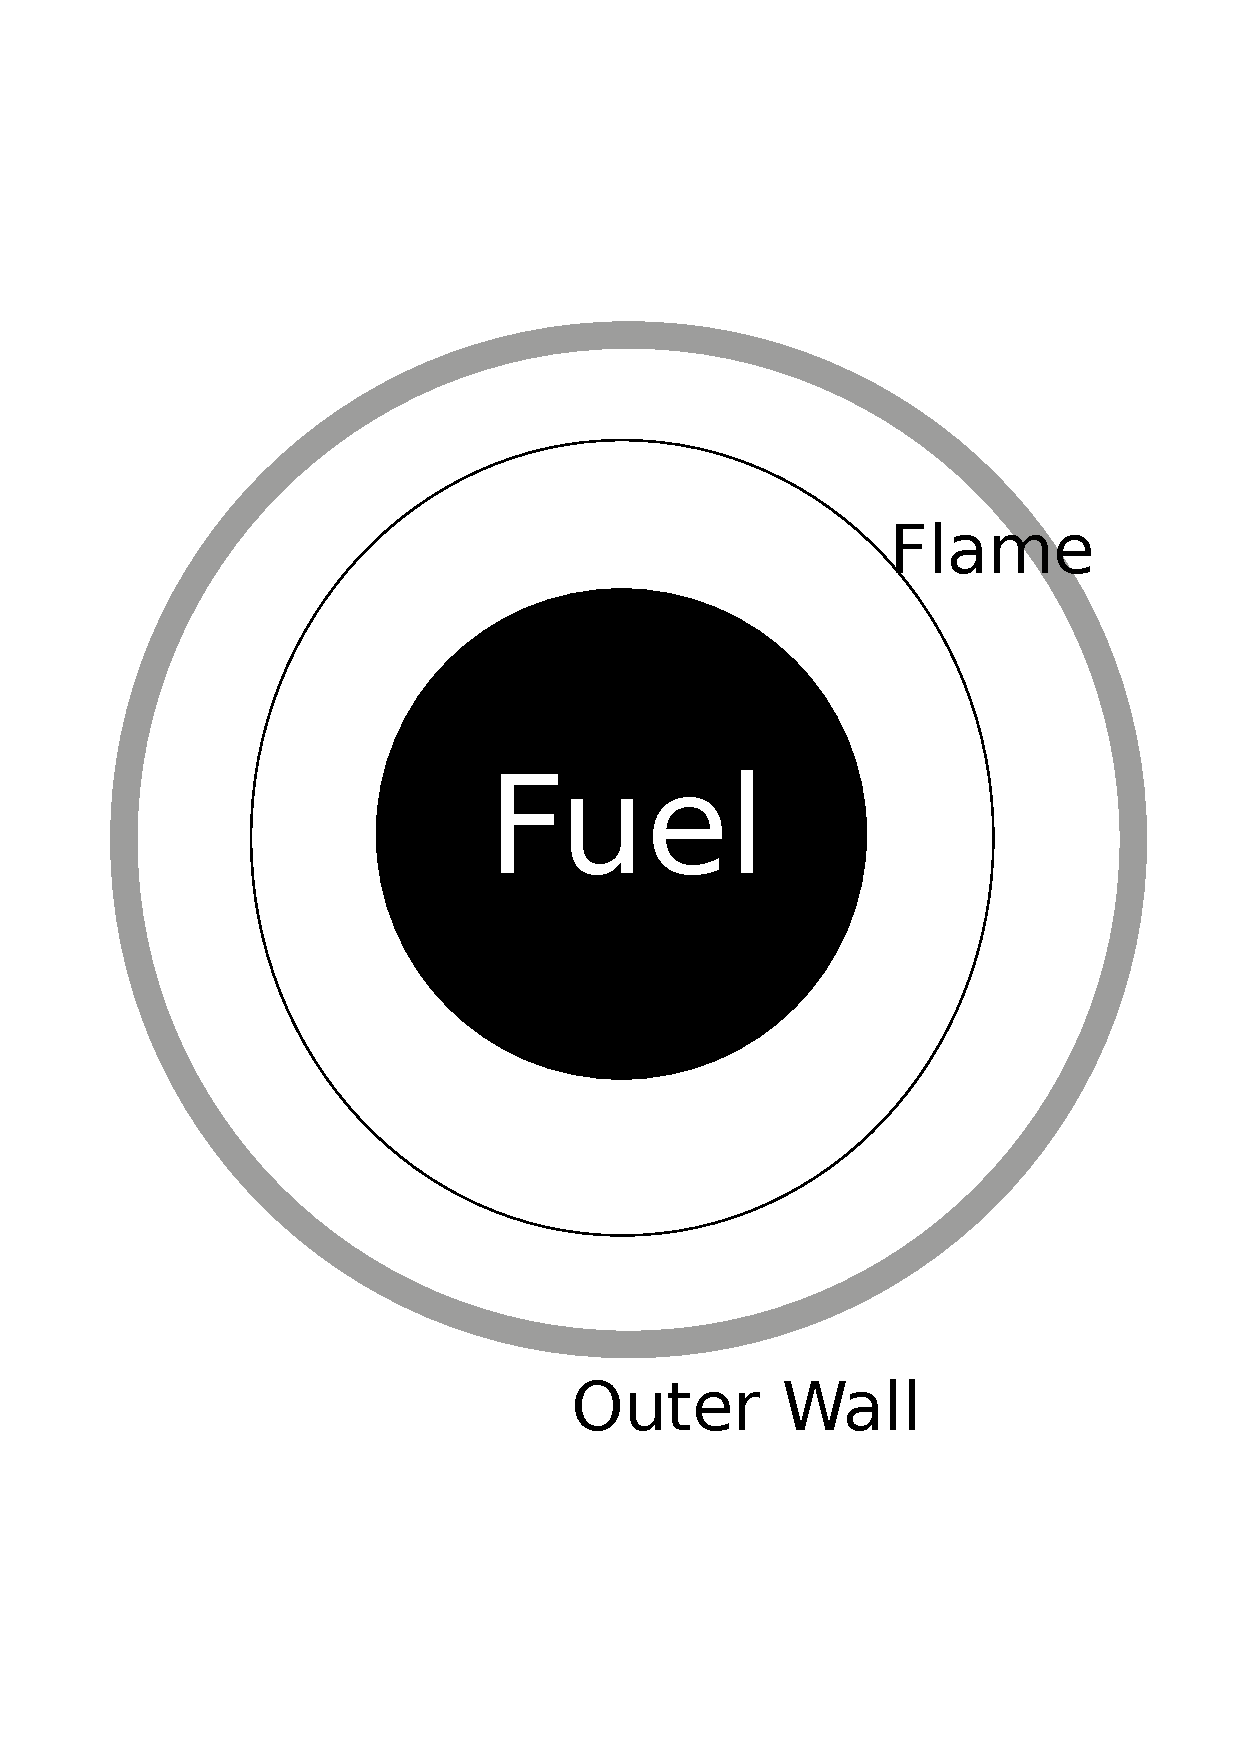
\includegraphics[scale=.3]{figs/spherical_burner.pdf}
  \caption{The spherical burner apparatus.}
 \end{center}
\end{figure}

The governing equation for the fuel is assumed to be, 
\begin{equation*}
 \frac{d}{dr}\left( r^2 \rho D \frac{dY_i}{dr}\right) = \pm r^2 w_i. 
\end{equation*}
Where, 
\begin{equation*}
 w_f = A Y_f Y_o e^{-E/RT}.
\end{equation*}
\begin{center}
\line(1,0){350}
\end{center}
We will solve this as a quasi-steady problem, in that we assume the fuel
at the center is not shrinking as a function of time. Note that, 
\begin{equation*}
\omega = \frac{\omega_i}{\nu_i W_i}= \frac{\omega_F}{\nu_F W_F} =
 \frac{\omega_O}{\nu_O W_O} 
\end{equation*}
This hints at a Shvab-Zel'dovich conserved scalar form that will
decouple the chemistry from the convection-diffusion of a conserved
scalar quantity. In particular, 
\begin{equation*}
\mathcal{L}\left(\beta \right) = \mathcal{L}\left( \frac{Y_O}{\nu_O W_O}
	    - \frac{Y_F}{\nu_F W_F} \right) \Rightarrow \frac{d}{dr}\left( r^2
	    \rho D \frac{d \beta}{dr}\right) = 0 .
\end{equation*}
Now, we must solve this equation. After the first integration, we have, 
\begin{equation*}
\frac{d \beta}{dr} = \frac{C_1}{ \rho D r^2 }.
\end{equation*}
This assumes constant density and transport properties. The second
integration in $r$ leaves us with, 
\begin{equation*}
\beta(r) = C_2 - \frac{C_1}{ \rho D r }.
\end{equation*}

The boundary conditions are stated as, ``the fuel and air diffuse from the walls
and are maintained at the walls with mass fraction of unity''. In other
words, $B(r_i) \rightarrow Y_f = 1, Y_O = 0 $ and $B(r_o) \rightarrow
Y_f = 0, Y_O = 1$. 

\newpage
\section*{Problem 2}



\end{document}
